%%%%%%%%%%%%%%%%%%%%%%%%%%%%%%%%
%%%
%%% Research Summary
%%%
%%% Author - Steve Hurder
%%%
%%% Date Started: October 12, 2009
%%% Date Completed: November 15 , 2009
%%%%%%%%%%%%%%%%%%%%%%%%%%%%%%%%

\documentclass[11pt]{amsart}
\usepackage{graphicx}
\usepackage{amssymb}
\usepackage{colortbl}
\usepackage{wrapfig}
\usepackage{epstopdf}
\usepackage{nicefrac}
\usepackage{url}


\usepackage[top=1in, bottom=1in, left=1in, right=1in]{geometry}

\newcommand{\student}[1]{\vspace{.5cm}\fbox{\parbox{0.95\linewidth}{{\small
        #1}}}\vspace{.5cm}}
\providecommand{\blue}[1]{{\color{blue}{#1}}}
\providecommand{\red}[1]{{\color{red}{#1}}}
\providecommand{\green}[1]{{\color{green}{#1}}}

\begin{document}

 \title{Machine Learning Shouldn't be a Black Box}

 \author{Jordan Boyd-Graber, CU Boulder}
%\institute{University of Colorado, Boulder CO 80309, USA}
\email{jbg@boydgraber.org}

%\date{March 14, 2013}

\maketitle

Machine learning is ubiquitous: detecting spam e-mails, flagging fraudulent
purchases, and providing the next movie in a Netflix binge.  But few users at
the mercy of machine learning \emph{outputs} know what's happening behind the
curtain.  My research goal is to demystify the black box for non-experts by
creating \emph{algorithms that can inform, collaborate with, compete with, and
  understand users} in real-world settings.

This is at odds with mainstream machine learning---take topic models.  Topic
models are sold as a tool for understanding large data collections: lawyers
scouring Enron e-mails for a smoking gun, journalists making sense of Wikileaks,
or humanists characterizing the oeuvre of Lope de Vega.  But topic models'
proponents never asked what those lawyers, journalists, or humanists
needed. Instead, they optimized \emph{held-out likelihood}. When my colleagues
and I developed the \emph{interpretability} measure to assess whether topic
models' users understood their outputs, we found that interpretability and
held-out likelihood were negatively correlated~\cite{chang-09b}! The topic
modeling community (including me) had fetishized complexity at the expense of
usability.

\begin{center}
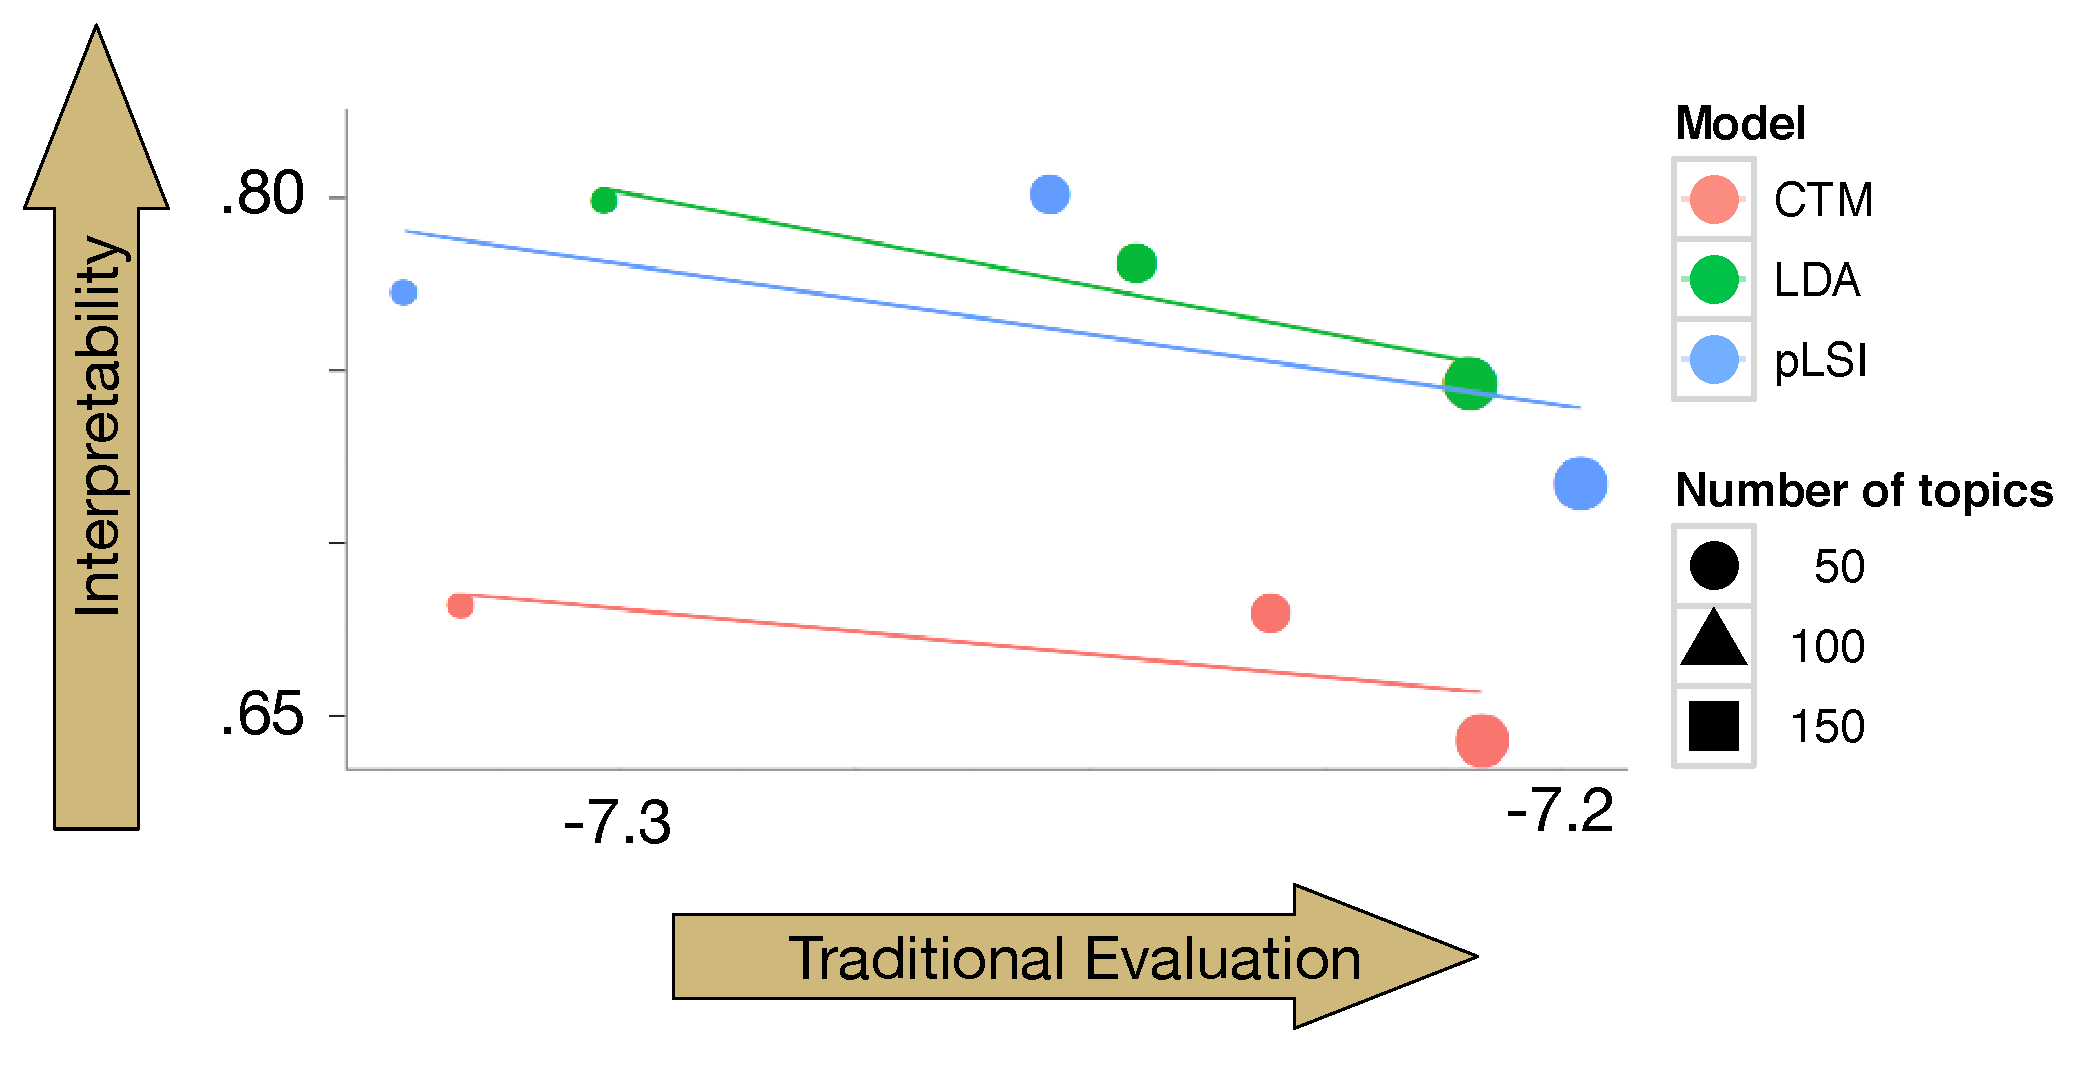
\includegraphics[width=.5\linewidth]{images/prec_ll_4}
\end{center}

Since this humbling discovery, I've built topic models that are a collaboration
between humans and computers.  The computer starts by proposing an organization
of the data.  The user responds by separating confusing clusters, joining
similar clusters together, or comparing notes with another
user~\cite{hu-14:itm}.  The model updates and then directs the user to
problematic areas that it knows are wrong.  This is a huge improvement over the
``take it or leave it'' philosophy of most machine learning algorithms.

This is not only a technical improvement but also an improvement to the social
process of machine learning adoption. A program manager who used topic models to
characterize \textsc{nih} investments uncovered interesting synergies and
trends, but the results were unpresentable because of a fatal flaw: one of the
700 clusters lumped urology together with the nervous system, anathema to
\textsc{nih} insiders~\cite{talley-11}. Our tools allow non-experts to fix such
obvious problems (obvious to a human, that is), allowing machine learning
algorithms to overcome the \emph{social} barriers that often hamper adoption.

\begin{minipage}[b]{0.4\textwidth}
\begin{tabular}{p{.9\textwidth}}
	Topic Words (before) \\
\hline
 \red{bladder}, sci, \blue{spinal\_cord}, \blue{spinal\_cord\_injury}, \blue{spinal}, \red{urinary}, \red{urinary\_tract}, \red{urothelial},\blue{injury}, \blue{motor}, \blue{recovery}, \blue{reflex}, \blue{cervical}, \red{urothelium}, \blue{functional\_recovery} \\
\end{tabular}
\end{minipage}
  \hfill
\begin{minipage}[b]{0.4\textwidth}
\begin{tabular}{p{.9\textwidth}}
	Topic Words (after) \\
\hline
sci, \blue{spinal\_cord}, \blue{spinal\_cord\_injury}, \blue{spinal}, \blue{injury}, \blue{recovery}, \blue{motor}, \blue{reflex}, \red{urothelial}, \green{injured}, \blue{functional\_recovery}, \green{plasticity}, \green{locomotor}, \blue{cervical}, \green{locomotion}\\
\end{tabular}
\end{minipage}

% Fix ``on the fly''

Our realization that humans have a lot to teach machines led us to
\emph{simultaneous machine
  interpretation}~\cite{Grissom:He:Boyd-Graber:Morgan-2014}. Because verbs end
phrases in many languages, such as German and Japanese, existing algorithms must
wait until the end of a sentence to begin translating (since English sentences
have verbs near the start). We learned tricks from professional human
interpreters---passivizing sentences and guessing the verb---to translate
sentences sooner~\cite{He-15}, letting speakers and algorithms cooperate together and
enabling more natural cross-cultural communication.

The reverse of cooperation is competition; it also has much to teach
computers. I've increasingly looked at language-based games whose clear goals
and intrinsic fun speed research progress.  For example, in \emph{Diplomacy},
users chat with each other while marshaling armies for world conquest.
Alliances are fluid: friends are betrayed and enemies embraced as the game
develops. However, users' conversations let us predict when friendships break:
betrayers writing ostensibly friendly messages before a betrayal become more
polite, stop talking about the future, and change how much they
write~\cite{niculae-15}.  Diplomacy may be a nerdy game, but it is a fruitful
testbed to teach computers to understand messy, emotional human interactions.

A game with higher stakes is politics.  However, just like Diplomacy, the words
that people use reveal their underlying goals; computational methods can help
expose the ``moves'' political players can use.  With collaborators in political
science, we've built models that: show when politicians in debates strategically
change the topic to influence others~\cite{nguyen-12,Nguyen-14b}; frame topics
to reflect political leanings~\cite{nguyen-13:shlda}; use subtle linguistic
phrasing to express their political leaning~\cite{iyyer-14a}; or create
political subgroups with larger political
movements~\cite{Nguyen:Boyd-Graber:Resnik:Miler-2015}.

Conversely, games also teach humans \emph{how computers think}.  Our
trivia-playing robot~\cite{boyd-graber-12,iyyer-14b,iyyer-15} faced off against
four former Jeopardy champions in front of 600 high school
students.\footnote{\url{https://www.youtube.com/watch?v=LqsUaprYMOw}} The
computer claimed an early lead, but we foolishly projected the computer's
thought process for all to see.  The humans learned to read the algorithm's
ranked dot products and schemed to answer just before the computer. In five
years of teaching machine learning, I've never had students catch on so quickly
to how linear classifiers work.  The probing questions from high school students
in the audience showed they caught on too.  (Later, when we played again against
Ken Jennings,\footnote{\url{https://www.youtube.com/watch?v=kTXJCEvCDYk}} he sat
in front of the dot products and our system did much better.)

  \begin{minipage}[b]{0.4\textwidth}
    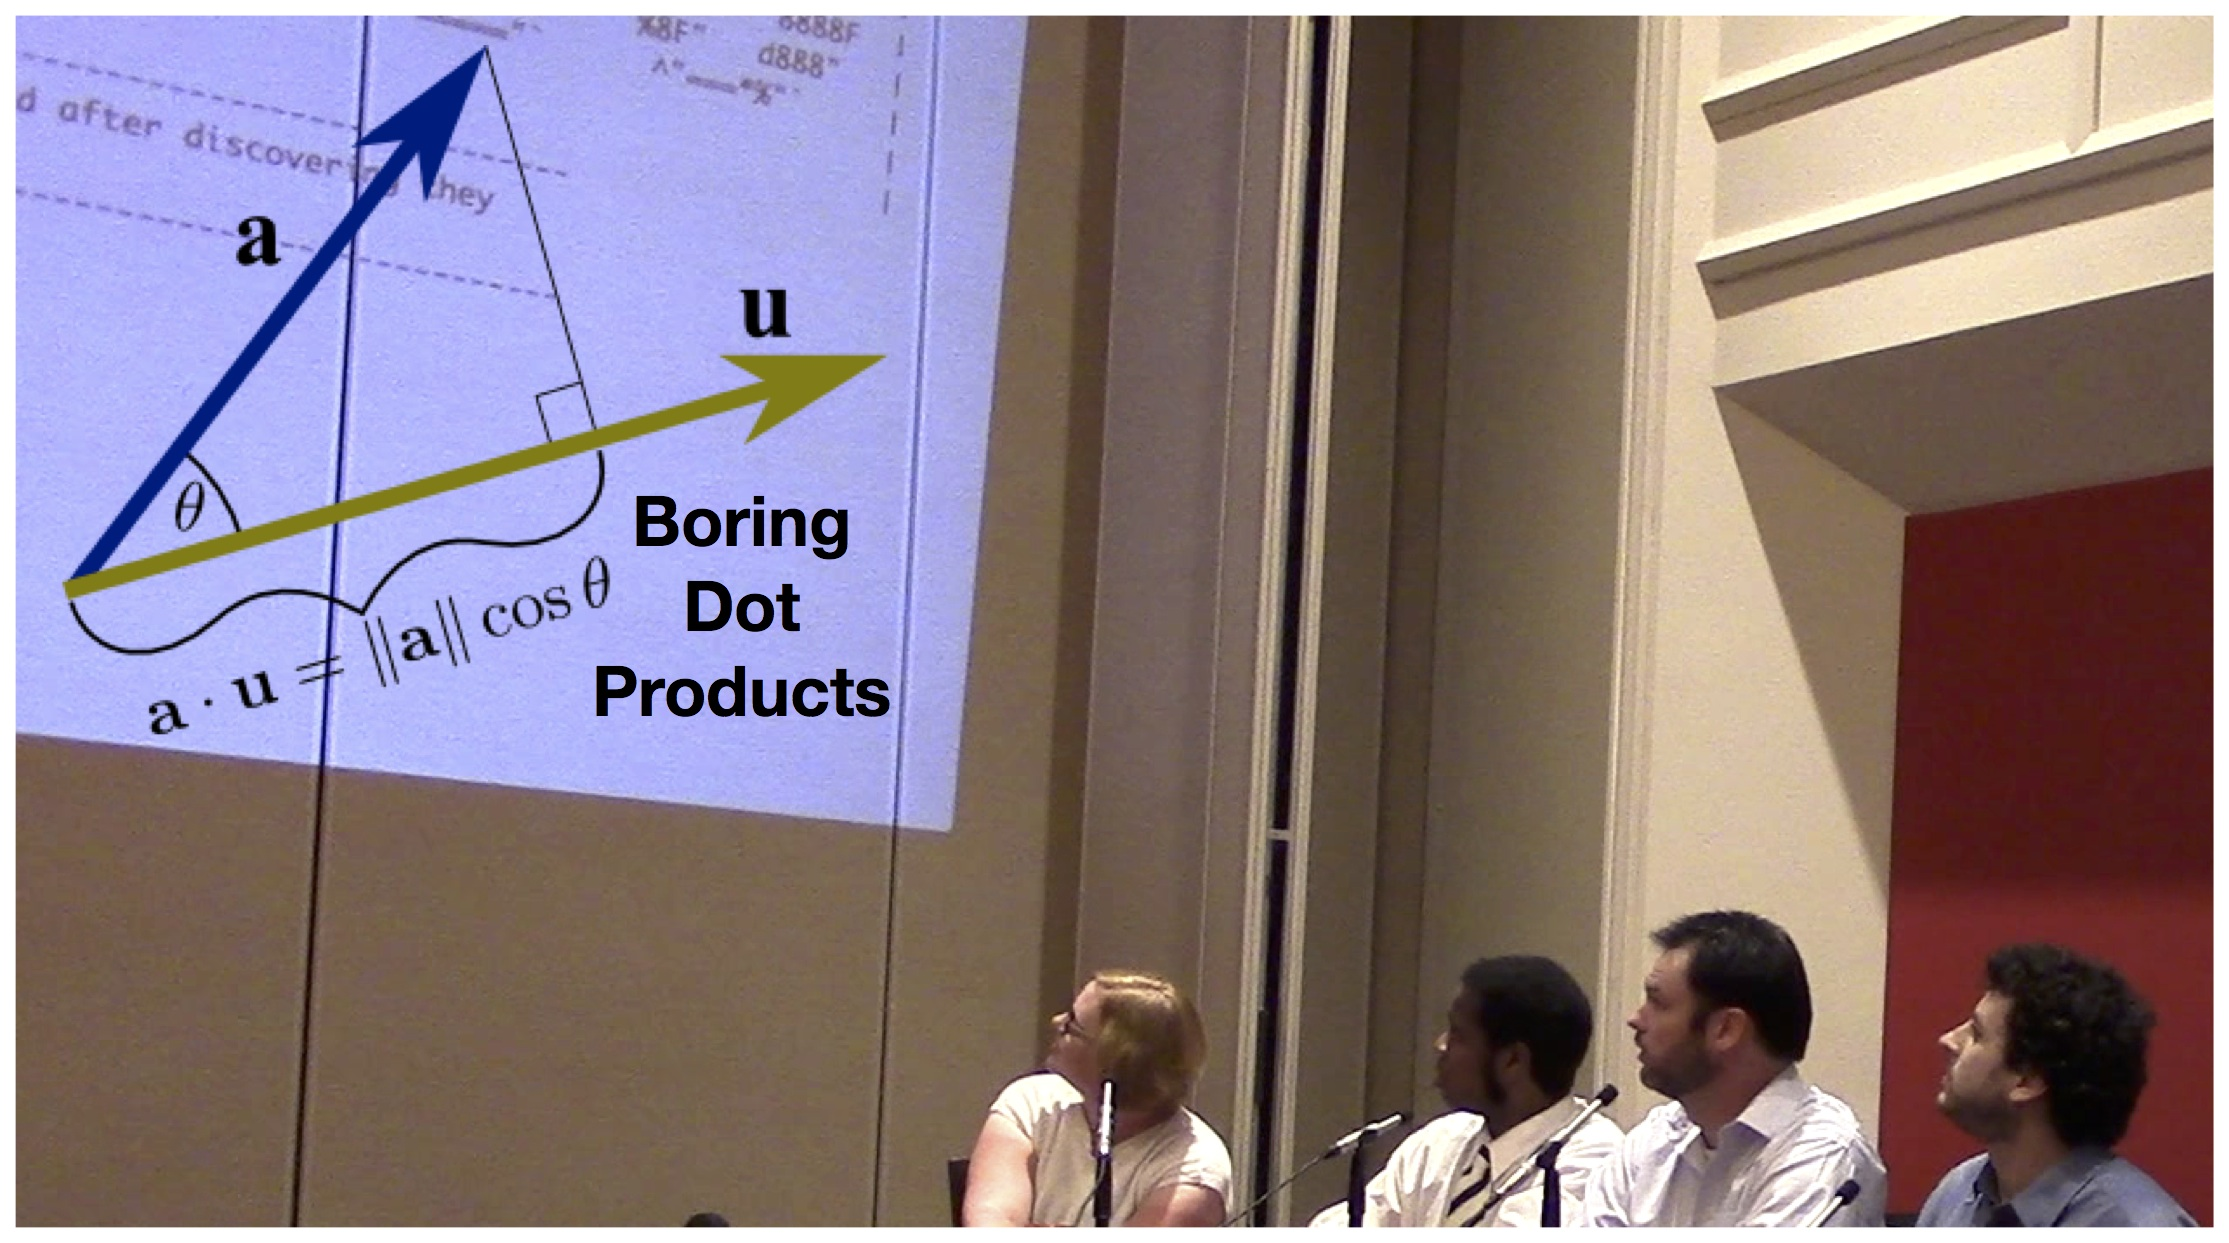
\includegraphics[width=\textwidth]{images/boring_dot_products}
  \end{minipage}
  \hfill
\begin{minipage}[b]{0.4\textwidth}
    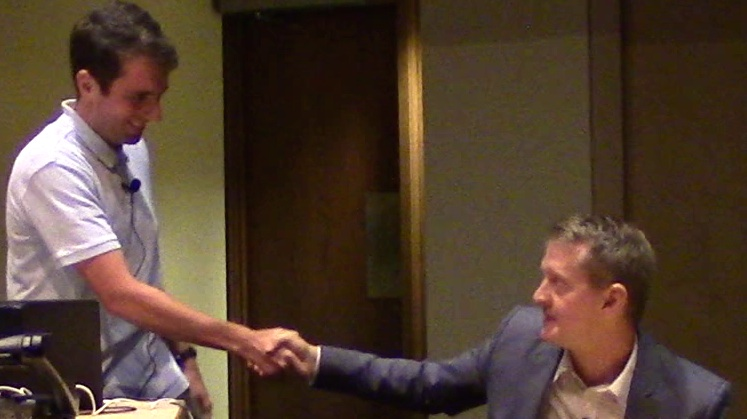
\includegraphics[width=\textwidth]{images/jennings_handshake}
  \end{minipage}


Advancing machine learning requires closer, more natural interactions.  However,
we still require much of the user---reading distributions or dot
products---rather than natural language interactions.  Document exploration
tools should describe in words what a cluster is, not just provide inscrutable
word clouds; deception detection systems should say \emph{why} a betrayal is
imminent; and question answers should explain \emph{how} it knows Aaron Burr
shot Alexander Hamilton. My work will complement machine learning's ubiquity
with transparent, empathetic, and useful interactions with users.
\clearpage
%%%%%%%%%%%%%%%%%%%%%%%%%%%%%%%%
\small
\bibliographystyle{resume_src/splncs03}

\begin{center}
Full list of  three book chapters, six journal publications, and fifty-five conference
publications at \url{http://boydgraber.org/dyn-pubs/year.html}
\end{center}

%\bibliographystyle{unsrtnat}
\bibliography{resume_src/journal-full,resume_src/jbg}
\noindent\rule{4cm}{0.4pt}
\end{document}
